\section{Rasterisation and anti-aliasing}
\label{sec:raster}
\here{7}
Rasterisation finds the pixels whose centres a triangle covers (edge functions) and interpolates the
vertex attributes with barycentric weights. Because the triangle was projected, attributes must be interpolated
perspective-correctly: interpolate $a/w$ and $1/w$, then divide.
\begin{equation}
E_{ij}(\vect x)=(\vect x-\vect p_i)\times(\vect p_j-\vect p_i),\quad
\lambda_k=\frac{E_k}{E_0+E_1+E_2},\qquad
a=\frac{\sum_k\lambda_k a_k/w_k}{\sum_k\lambda_k/w_k}
\label{eq:raster}
\end{equation}
\begin{itemize}
\item Edge function of the directed edge $\vect a\to\vect b$ at $\vect p$: $E=(b_x-a_x)(p_y-a_y)-(b_y-a_y)(p_x-a_x)$, twice the
signed area of $(\vect a,\vect b,\vect p)$; $\sum_kE_k$ is twice the triangle's area, so the $\lambda_k$ sum to 1.
\item Top-left rule: a pixel centre exactly on an edge belongs to the triangle only if that edge is a top or left edge,
so two triangles sharing an edge never both draw (or both miss) its pixels.
\item The \ab{519}{GPU} does this in hardware; \code{math/ExplorerMath.cpp: rasterize} and \code{interpolatePerspective} compute the
same numbers for the Frame Explorer (Listing below, Figure~\ref{fig:raster}).
\end{itemize}
\begin{lstlisting}[language=C++,caption={Edge functions, barycentric weights, perspective-correct interpolation (\code{math/ExplorerMath.cpp}).}]
float edgeFunction(const Vec2f& a, const Vec2f& b, const Vec2f& p) {
    return (b.x - a.x) * (p.y - a.y) - (b.y - a.y) * (p.x - a.x);
}
b.e0 = edgeFunction(v1, v2, p);  b.e1 = edgeFunction(v2, v0, p);  b.e2 = edgeFunction(v0, v1, p);
const float area2 = signedArea2(v0, v1, v2);
b.w0 = b.e0 / area2;  b.w1 = b.e1 / area2;  b.w2 = b.e2 / area2;   // lambda_k
float interpolatePerspective(const Barycentric& b, float w0, float w1, float w2, float a0, float a1, float a2) {
    const float num = b.w0 * a0 / w0 + b.w1 * a1 / w1 + b.w2 * a2 / w2;
    const float den = b.w0 / w0 + b.w1 / w1 + b.w2 / w2;
    return den != 0.0f ? num / den : 0.0f;
}
\end{lstlisting}

\textbf{Lines: \ab{520}{DDA} and Bresenham.} Wireframes, hidden-line edges and debug paths are \code{GL\_LINES} drawn by the
\abp{521}{GPU} line rasteriser; the two textbook line algorithms (Figure~\ref{fig:aa-plots}c) step one pixel at a time:
\begin{gather}
\text{DDA: } x_{i+1}=x_i+1,\quad y_{i+1}=y_i+m,\quad m=\frac{\Delta y}{\Delta x},\quad \text{plot }\big(x_i,\operatorname{round}(y_i)\big)\label{eq:lines}\\
\text{Bresenham: } p_0=2\Delta y-\Delta x,\qquad p_{i+1}=\begin{cases}p_i+2\Delta y & p_i<0\\ p_i+2\Delta y-2\Delta x & p_i\ge0\quad (y\gets y+1)\end{cases}\nonumber
\end{gather}
The same incremental idea walks a ray through the terrain's height-field grid in the ray tracer (a 3D \ab{522}{DDA},
\code{raytrace/Heightfield.cpp}): $t_{\max,x}\gets t_{\max,x}+\Delta t_x$ with $\Delta t_x=\text{cell}/|d_x|$, stepping
the axis whose next boundary is nearer.

\begin{figure}[htbp]
\centering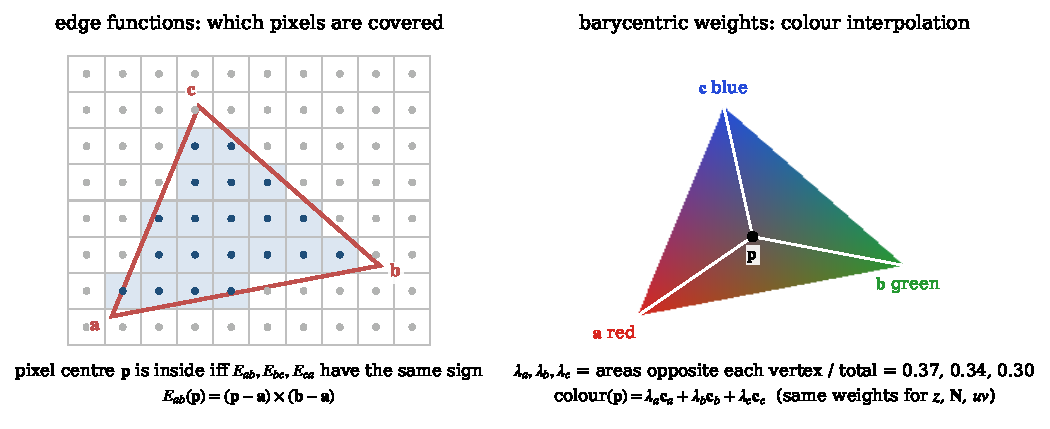
\includegraphics[width=\linewidth]{figures/diagrams/d_raster.pdf}
\caption{Rasterisation and colour interpolation.}
\label{fig:d-raster}
\end{figure}

\begin{figure}[htbp]
\centering
\begin{subfigure}[t]{0.49\linewidth}\raw{lab/explorer_raster_scan}{\linewidth}\caption{Frame Explorer: the raster scan of one triangle.}\end{subfigure}\hfill
\begin{subfigure}[t]{0.49\linewidth}\raw{lab/explorer_interp_affine_perspective}{\linewidth}\caption{Affine (left) vs perspective-correct (right).}\end{subfigure}
\\[1mm]
{\footnotesize\textit{Zoomed panels of the Frame Explorer frame:}}\\[0.5mm]
\feRasterScanInfo\hfill\feInterpAffinePerspectiveInfo
\caption{Rasterisation in the Frame Explorer: (a) the scan of one triangle; (b) the affine checker bends along each
quad's diagonal, the perspective-correct one stays straight.}
\label{fig:raster}
\end{figure}

\textbf{Anti-aliasing.} Edges sampled once per pixel form stairs. The program uses \ab{523}{MSAA} (several coverage samples, one
shading per pixel): 2$\times$ at LOW, 4$\times$ at HIGH, 8$\times$ at ULTRA and 4$\times$ at EPIC, with \ab{524}{TAA} from HIGH up (Table~\ref{tab:aa}). \ab{525}{TAA}
jitters the projection by a Halton(2,3) sub-pixel offset every frame and blends the history, clipped to the
variance box of the current $3\times3$ neighbourhood in YCoCg. The affine checker of Figure~\ref{fig:raster}b bends
because $a$ is interpolated linearly in screen space instead of through $a/w$.
\begin{gather}
\text{MSAA: } c_{\text{pixel}}=\frac1n\sum_{i=1}^{n}c\big(\text{triangle covering sample } i\big),\qquad n\in\{2,4,8\}\label{eq:aa}\\
\text{jitter: } \delta_k=\Big(\frac{2(h_2(k)-\frac12)}{W},\ \frac{2(h_3(k)-\frac12)}{H}\Big),\quad k=1..8\nonumber\\
\text{TAA: } c_t=\beta\,\operatorname{clip}(h_{t-1})+(1-\beta)\,x_t,\quad \beta=0.9\ (\text{still})\ \ldots\ 0.75\ (\text{fast motion})\nonumber\\
\operatorname{clip}: \text{ towards } \mu \text{ into the box } \mu\pm1.1\,\sigma \text{ of the } 3\times3 \text{ neighbourhood (in YCoCg)}\nonumber
\end{gather}
\begin{itemize}
\item $h_b(k)$ is the radical inverse of $k$ in base $b$ (Halton): $h_2(1..4)=\frac12,\frac14,\frac34,\frac18$.
The offset is added to $P_{13}$ and $P_{23}$ of the projection, which moves the whole image by a sub-pixel amount.
\item The history weight $\beta^k$ decays geometrically (Figure~\ref{fig:aa-plots}b): an average over about
$1/(1-\beta)=10$ frames when still.
\item Code: jitter in \code{RendererFrame.cpp} (\code{halton}), blend and clip in \code{ShadersPostFx.cpp} (\code{kTaaFrag});
\ab{526}{MSAA} samples are resolved by the \ab{527}{GPU} (\code{glBlitFramebuffer}).
\end{itemize}

\begin{figure}[htbp]
\centering\plot{p_antialias}{\linewidth}
\caption{(a) The eight Halton(2,3) sub-pixel offsets of the TAA (temporal anti-aliasing) jitter; (b) weight of each past frame in the TAA history
for $\beta=0.9$ and 0.75 (Eq.~\eqref{eq:aa}); (c) the pixels DDA (digital differential analyser) and Bresenham choose for one line (Eq.~\eqref{eq:lines}):
the same set for this slope.}
\label{fig:aa-plots}
\end{figure}

\begin{table}[htbp]
\caption{Anti-aliasing per quality preset (\code{RendererFrame.cpp: qualityProfile}). Short forms: MSAA: multisample anti-aliasing; PCF: percentage-closer filtering; TAA: temporal anti-aliasing.}\label{tab:aa}
\centering\small
\begin{tabular}{@{}lllll@{}}
\toprule
 & LOW & HIGH & ULTRA & EPIC\\\midrule
MSAA samples $n$ & 2 & 4 & 8 & 4\\
TAA & off & on & on & on\\
Shadow PCF taps & 8 & 8 & 16 & 16\\
\bottomrule
\end{tabular}
\end{table}

\begin{figure}[htbp]
\centering\raw{lab/explorer_stage_15_taa}{0.7\linewidth}
\\[1mm]
{\footnotesize\textit{Zoomed panels of the Frame Explorer frame:}}\\[0.5mm]
\feStageTaaInfo\hfill\feStageTaaFormula
\caption{Frame Explorer TAA (temporal anti-aliasing) stage: thin wires and grass blades stay continuous instead of breaking into dots.}
\label{fig:taa}
\end{figure}

Figure~\ref{fig:flow-raster} and Algorithm~\ref{alg:raster} follow one triangle through these steps.
\flowRaster
\algRaster

\textbf{Limitation.} \ab{528}{TAA} trades aliasing for blur and ghosting: a fast \ab{529}{UAV} leaves a faint trail for a few frames. With
a static camera, pixels without vegetation still change by about 2.4/255 per frame from the jitter alone and vegetation
pixels by 2.6--6.6/255, above the 1.5/255 that was the target.
